\chapter{Model automobilu}
\label{sec:CarModel} \

V této kapitole je popsán model automobilu a jeho jednotlivé části.

Model automobilu je založen na platformě Alamak, která má
\textbf{2 servomotory} pro otáčení předních kol a
\textbf{2 PWM motory} pro řízení každého
zadního kola.

\textbf{Platforma Alamak} je řízená pomocí \textbf{NXP Freedom K66F}\cite{frdmk66UserGuide} spolu
s modulem \textbf{POLI-TFC} přípojeným do GPIO pinů mikrokontroleru.
Detailní popis mikrokontroleru a modulu jsou v podkapitolách \ref{sec:FRDM-K66F}
a \ref{sec:POLI-TFC}.

Pro komunikaci s platformou Alamak je použit \textbf{WiFi Access Point}, který je připojen k MCU
pomocí Ethernet portu.

\textbf{Řádková kamera}, která umístěna v přední části platformy,
se používá pro získání obrazu drahy.

Vše je napojeno pomocí baterie typu \textbf{NiMH} o napětí 7.2V.

Celý model je zobrazen na obrázku \ref{fig:car}.
\begin{figure}[h]
    \centering
    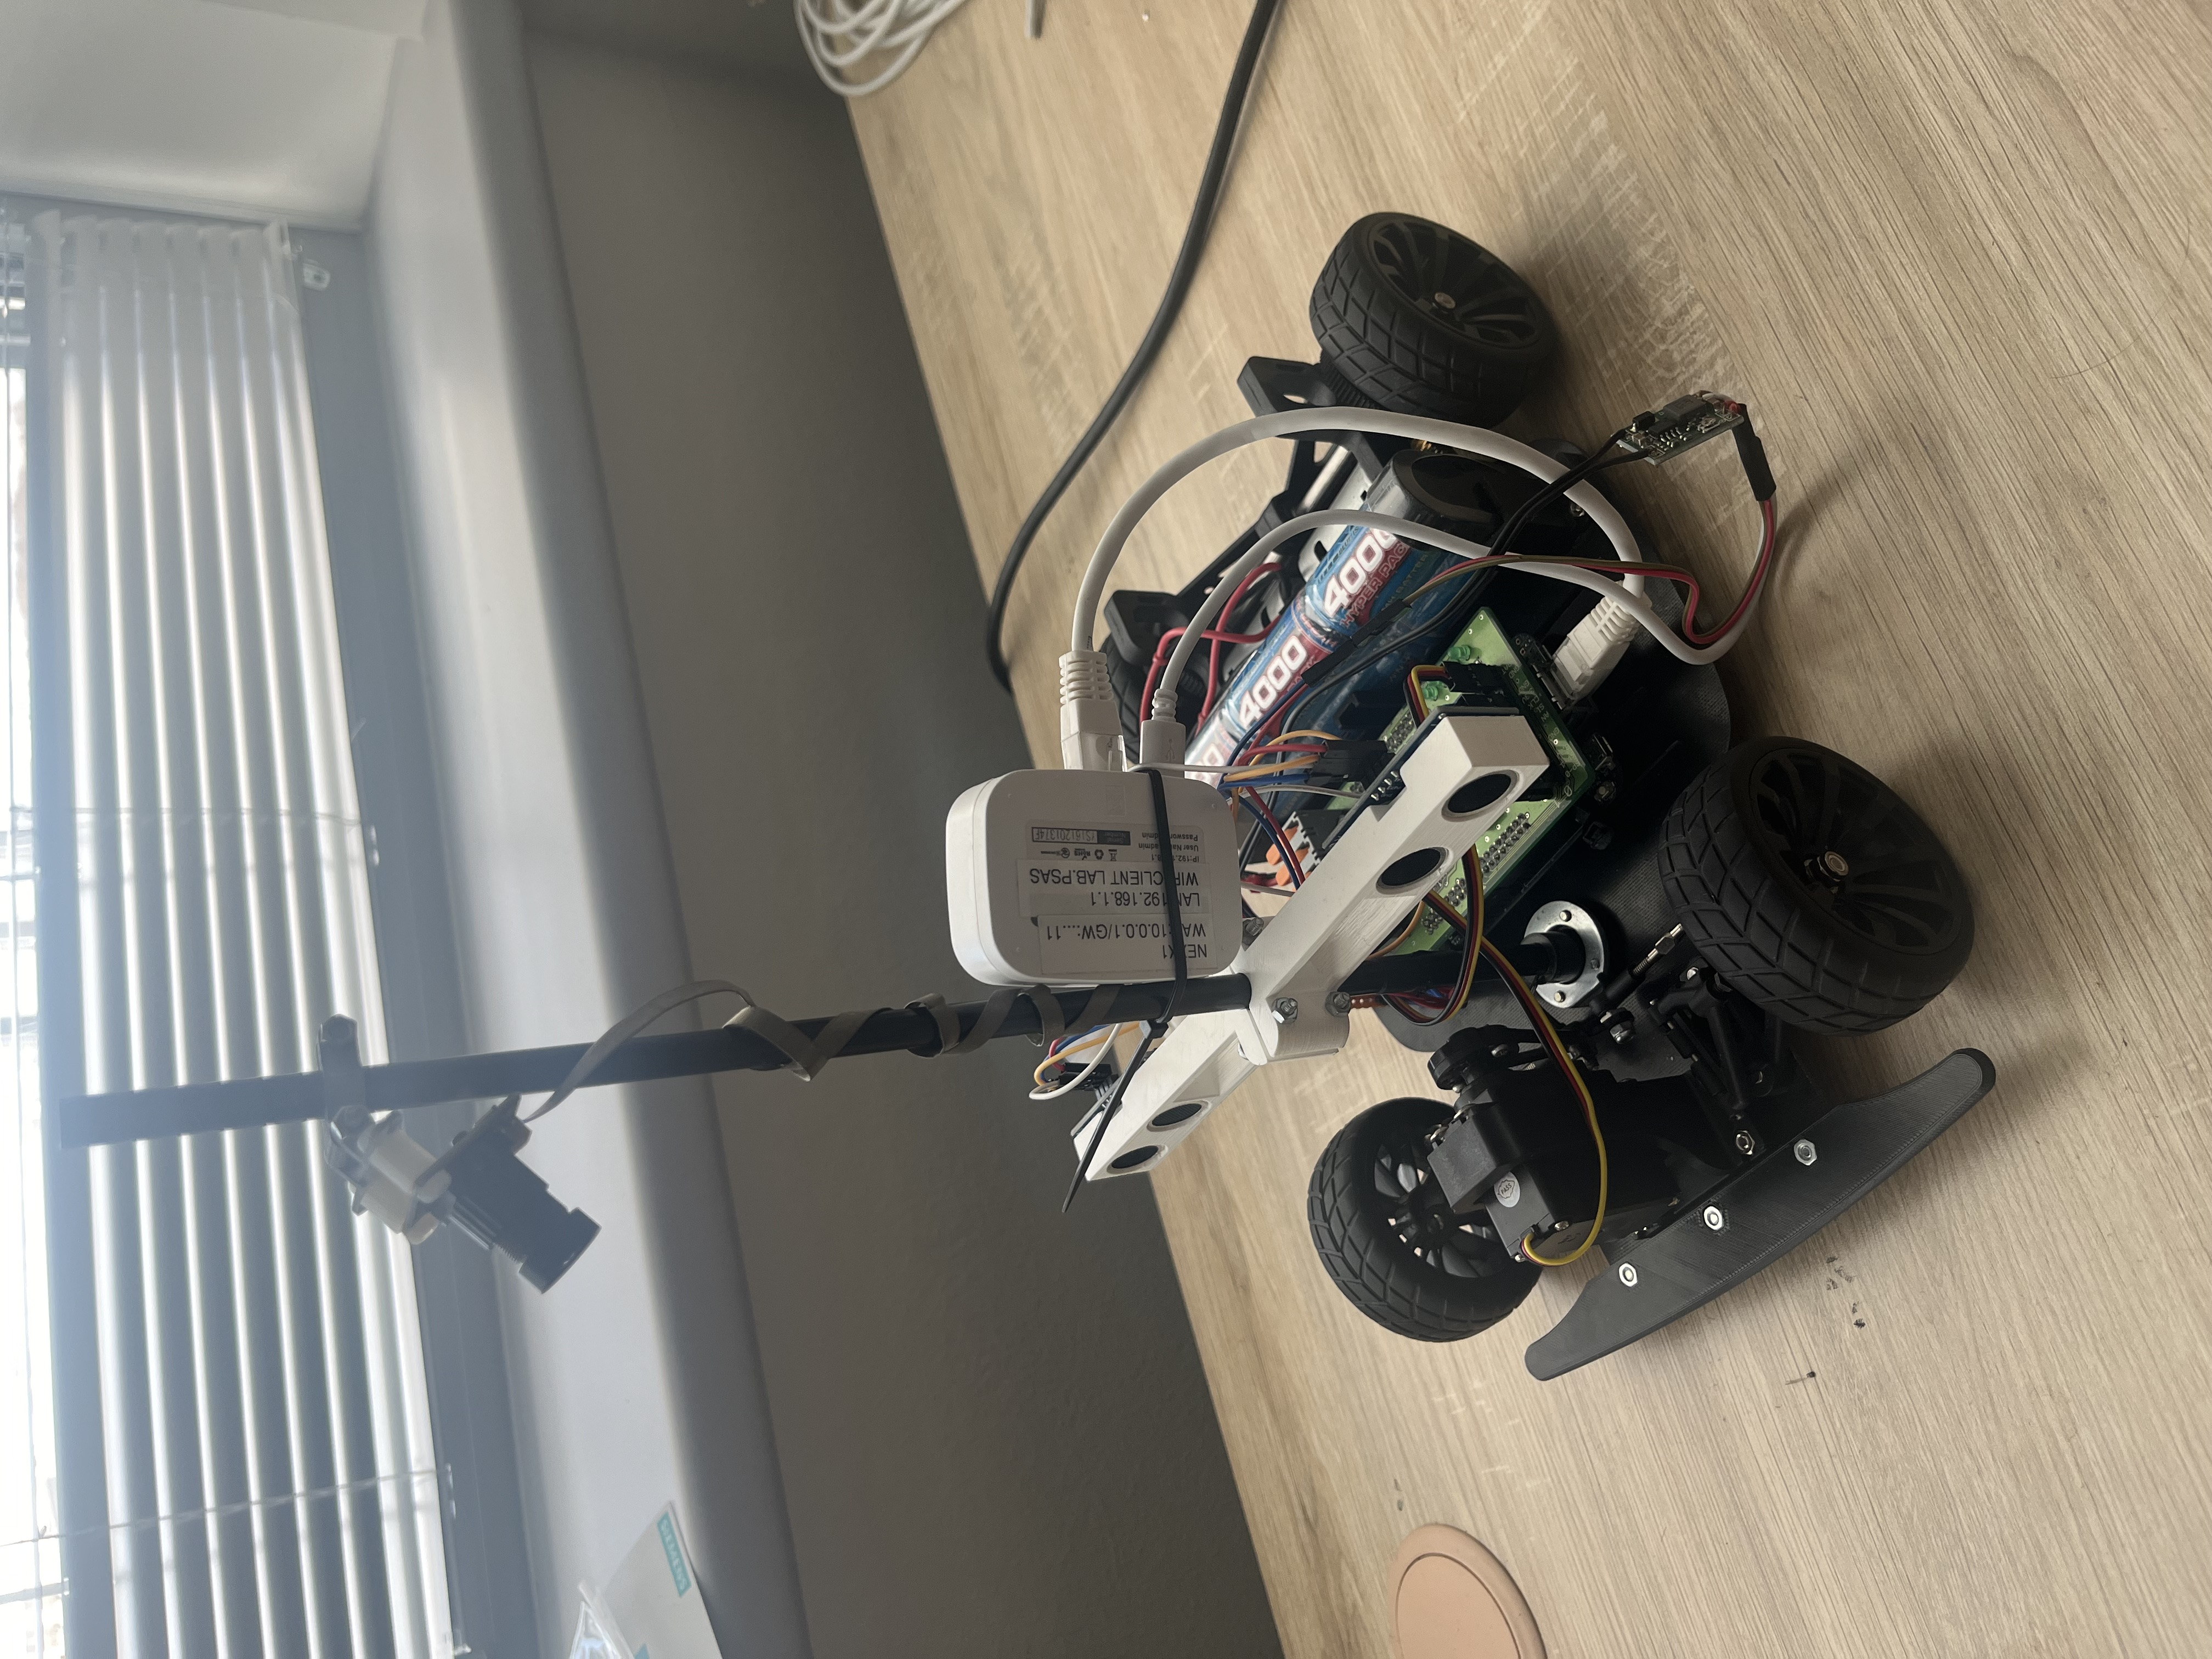
\includegraphics[width=0.45\linewidth, angle=-90]{Figures/car.jpeg}
    \caption{Model auta}
    \label{fig:car}
\end{figure}

\section{Mikrokontroler FRDM-K66F}
\label{sec:FRDM-K66F}
FRDM-K66F je vývojová platforma od společnosti NXP určená pro mikrokontroléry řady Kinetis K66 a K26.
Platforma je založena na jádře ARM© Cortex®-M4 a
konkrétně využívá model MK66FN2M0VMD18 s frekvencí 180 MHz, 2 MB flash paměti a 256 KB RAM.

Pro konektivitu platforma nabízí 2 micro-B USB porty, 1 ethernetový port a 54 GPIO konektorů.
GPIO piny jsou kompatibilní s Arduino™ R3, což poskytuje širokou škálu možností pro rozšiřující desky.
Pro další možnosti konektivity je deska vybavena moduly Bluetooth a RF.

Pro ladění je na platformě přítomno rozhraní OpenSDAv2.1, které podporuje J-Link.

Další užitečné periferie na desce zahrnují trojbarevnou LED, SDHC a digitální MEMS mikrofon.

Jako jednotku IMU platforma využívá akcelerometr společně s magnetometrem FXOS8700CQ
a gyroskop FXAS21002. Detailní popis jednotky je uveden v kapitole X.\cite{frdmk66UserGuide}

Vývojová platforma je znázorněna na obrázku.

\section{POLI-TFC}
\label{sec:POLI-TFC}
POLI-TFC shield je rozšiřující deska pro FRDK-K66F, která sjednocuje rozhraní pro
připojení periferií k vývojové desky. Shield obsahuje 2 konektoru pro PWM motory, 2 servomotoru,
2 rozhraní pro připojení řádkových kamer, 2 potenciometry, 4 DIP přepinače a 4 LED diody.
Shield je zobrazen na obrazku.
\endinput
